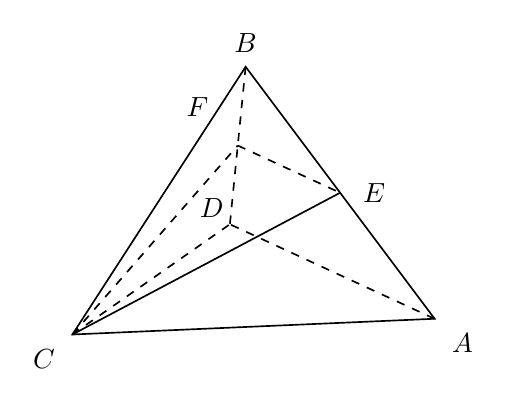
\begin{tikzpicture}[x=1cm,y=1cm,line width=.6pt,font=\normalsize,
geometry edge/.style={solid,line width=.6pt},
geometry label/.style={font=\normalsize,inner sep=2pt}]
\coordinate (B) at (2.2,3.4);
\coordinate (C) at (0,0);
\coordinate (A) at (4.6,0.2);
\coordinate (D) at (2.0,1.4);
\coordinate (E) at (3.4,1.8);
\coordinate (F) at (2.1,2.4);
% E is midpoint of B-A, F midpoint of B-D (computed)
% outer tetra solid
\draw[geometry edge] (B) -- (C) -- (A) -- cycle;

% median C-E solid
\draw[geometry edge] (C) -- (E);
% hidden edges dashed
\draw[geometry edge,dashed] (B) -- (D);
\draw[geometry edge,dashed] (C) -- (D);
\draw[geometry edge,dashed] (A) -- (D);
\draw[geometry edge,dashed] (C) -- (F);
\draw[geometry edge,dashed] (F) -- (E);
\node[geometry label,above,yshift=3pt] at (B) {$B$};
\node[geometry label,below left,xshift=-4pt,yshift=-3pt] at (C) {$C$};
\node[geometry label,below right,xshift=4pt,yshift=-3pt] at (A) {$A$};
\node[geometry label,above left,xshift=0pt,yshift=0pt] at (D) {$D$};
\node[geometry label,right,xshift=6pt] at (E) {$E$};
\node[above left=2pt,xshift=-5pt,yshift=5pt] at (F) {$F$};
\end{tikzpicture}
